\section{Protocols and Eligibility}
\subsection{Complete final-analysis protocols}
Cross-architecture sharing compares $A_0/B_0$ and identical $A_0/B_2$ for every ordered $A\ne B$ among HAT, SwinIR, I3Net, SAINT-style and CycleINR-style. No TTA is used. fastMRI targets are $\{3,5,7,9,11\}$; IXI uses the unchanged deterministic residue-balanced geometry. Both conditions use the same target-derived 1\% support. Five-plane means form examination observations. Primary $\Delta O$ and secondary alignment/disagreement differences average examinations. Fixed-reference and condition-specific paired-error rankings correlate examination means separately. The two cohorts are not pooled.

The acquired-only probe selects three rounded interior quartiles of $[3,\mathrm{depth}-4]$, with geometry-only deduplication. Its six acquired offsets are $\{-3,-2,-1,+1,+2,+3\}$; the target is absent. A common Q1 offset and Q99--Q1 range use finite nonzero acquired intensities; normalized values are clipped to $[0,1]$. The mask is the union of the nearest acquired planes' 1\% foregrounds. Both mask and normalizer are fixed before perturbations and shared across contexts. The common normalizer itself is shared preprocessing. Empty or invalid inputs would remain excluded with reasons; no case was removed by outcome.

Reference $(-2,+2)$ is compared with $(-2,+1)$, $(-2,+3)$, $(-1,+2)$, $(-3,+2)$, $(-1,+1)$, $(-1,+3)$, $(-3,+1)$, $(-3,+3)$. The self-pair is absent. Four centered Rademacher fields use seeds 6101--6104 on the $256\times256$ input grid. Primary amplitude is .01; .005/.02/$-.01$ are all retained. FP32 without AMP/TF32, input/output clipping and resizing are fixed. Responses and hashes are saved before separate targets are accessed. Error outcomes use the same acquired support. Broad points pool contexts/planes; fixed-count rank residuals adjust span/asymmetry and examination. Examination resampling retains subordinate observations and reranks repeated observations. Weighted computations match direct bootstrap expansion.

Each HAT/SwinIR stratum passes only if all three alternative-versus-primary rank correlations reach the existing .85 threshold; .70 remains the historical catastrophic floor. The original six-stratum aggregate gate is NA without an acquired-only NingXia replication. The .90 threshold belongs to a separate historical new-architecture protocol and is not substituted here.

For the perturbation experiment, sort IXI IDs by SHA-256 of \texttt{MIRA-final-proposition:} plus ID and take the first twelve; use the depth-only central target, both models and all four exactly-one-anchor contexts. Perturb only the common anchor, holding other inputs, masks and scales fixed. Four fields and their negatives define eight equal-weight samples. Coupled outputs pair equal field indices; independent outputs average the entire Cartesian product, giving exactly equal empirical marginals. All amplitudes .0025/.005/.01/.02 remain. The odd response at .0025 supplies a fixed linear prediction scaled by squared amplitude. Relative error divides by the magnitude of that prediction. Reference response cosine $\ge.1$, $\le-.1$ and intermediate values label aligned, opposing and near-orthogonal examples descriptively, without eligibility selection.

All final intervals use 5,000 paired examination draws. Seeds are 18001/18002 for cross-architecture fastMRI/IXI; 18003/18004 for acquired-only IXI/fastMRI; 18005 for perturbation validation. Maximum standardized bootstrap deviation yields simultaneous intervals over 20 ordered pairs per cohort/endpoint, two models per acquired-only cohort/endpoint, or two models times four amplitudes. Pointwise intervals and finite-draw counts remain in the CSVs. These families do not correct the full retrospective search history.

\subsection{Objective Qualitative Selection and Precision Check}
The main example is selected from the historical complete fastMRI SwinIR table. Rank examinations by their mean disjoint-minus-shared observable gain, tie by ID, and take the lower median (12th of 24). Within that case select the target whose gain is nearest its case mean, tie by $z$. This produces case 103425595595, $z=9$. A separate seed-20260911 random draw from the other examinations produces case 101089005814, $z=7$. The full ranking and selection file were saved before CPU inference. Neither visual appearance nor a newly optimized stable-wrong threshold selects the examples.

\begin{figure*}[t]
\centering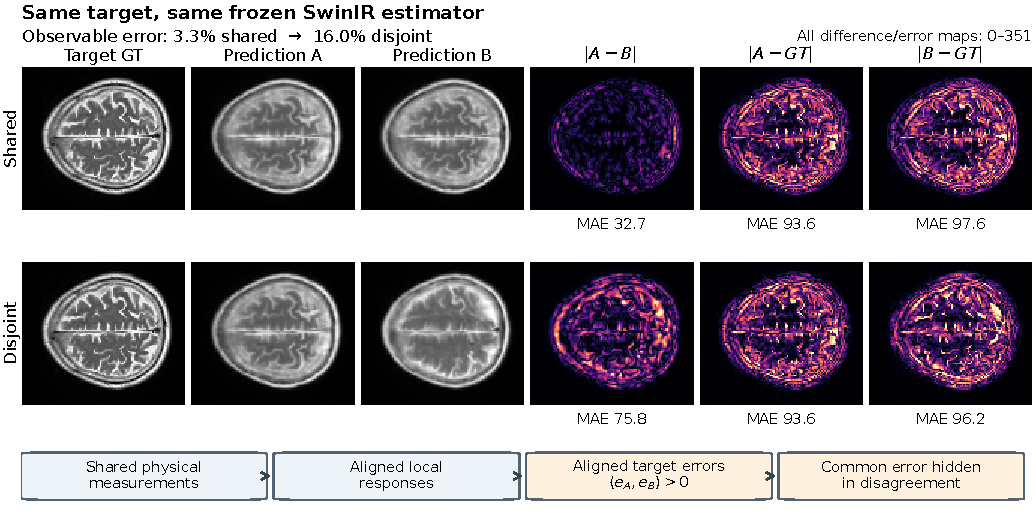
\includegraphics[width=.98\textwidth]{p17_qualitative_random.pdf}
\caption{Seeded random supplemental example under the same rendering rule as the main figure. All difference/error maps share a scale; there is no manually selected crop. The reference prediction and target are identical across rows. Shared and disjoint observable fractions are 3.34\% and 16.00\%. The schematic chain is conditional on aligned sensitivities and does not assert that every shared pair must fail.}
\label{fig:p17-random}
\end{figure*}

Both cases use the hashed historical SwinIR checkpoint with direct target inference using the original wrapper's context normalization, resizing and residual prediction. CPU float32 reference outputs differ from stored GPU mixed-precision outputs by MAE .118/.153 and maximum absolute difference 2.694/2.442 in native units. Thus no exact reproduction claim is made for these new illustrations. Observable fractions differ by less than $4.6\times10^{-5}$ from the historical table. Cohort statistics remain the original values. Original arrays, masks, common display ranges and selection hashes are retained.

\subsection{Definitions and Documented Protocol}
For predictions $f_a=y+e_a$ and $f_b=y+e_b$, shared and observable error fractions are
\begin{equation}
S=\frac{\|\bar e\|^2}{\|\bar e\|^2+\|\delta\|^2},\qquad
O=\frac{\|\delta\|^2}{\|\bar e\|^2+\|\delta\|^2},
\end{equation}
where $\bar e=(e_a+e_b)/2$ and $\delta=(e_a-e_b)/2$. Numerical identity error is below $4.42\times10^{-10}$ in the stored audit.

For nonlinear models, four frozen seeds (6101--6104) generate centered Rademacher fields at 1\% of the globally normalized case range. Each shared anchor is perturbed separately. The influence numerator sums identical-field response inner products over shared anchors and seeds, while its denominator uses the geometric mean of all-anchor response energies on the two sides, including unshared anchors. The broad grid uses reference offsets $(-2,+2)$ and eight target-preserving comparators. Span and asymmetry are explicit covariates; the complete offset list is stored with the experiment registry. The fixed-count subset contains the four comparators with exactly one common anchor.

\subsection{Plan-9 Architecture-Family Protocol}
The architecture hypothesis and falsification conditions are recorded in local documents; their pre-outcome timing is not independently established. Phase-0 anchors are $\{0,4,8,12\}$, phase-2 anchors are $\{2,6,10,14\}$, and common missing targets are $\{3,5,7,9,11\}$. The clean shared control applies an in-plane horizontal flip to phase-0 inputs and maps outputs back. A one-case smoke using through-plane reversal was rejected after its one-case outcome exposed order non-equivariance; documents report that this preceded full-cohort inference; its outputs are retained but excluded. Regenerated phase-0 outputs match stored predictions exactly for every one of 24 cases and all five architectures (pixel MAE and maximum absolute difference zero).

I3Net uses four regular anchors and outputs 13 planes. SAINT consumes a left/right pair plus relative and absolute position maps. The internal CycleINR-style model linearly densifies four regular anchors and queries a coordinate-conditioned residual network. The adapted SAINT and CycleINR-style implementations are not claimed as exact official reproductions. All interventions occur at physical anchor identity; no architecture is distorted into another input interface.

The following historical table preserves masked/common-support recovery, including its missing cells. Those missing cells do not mean the native baseline runs are absent: the complete native 13-model, three-cohort comparison and all 111 configurations are retained elsewhere in this supplement. The two supports are not interchangeable and no method is labeled ours.



